\documentclass{article}
\usepackage[utf8]{inputenc}
\usepackage[english]{babel}
\usepackage[font=small,labelfont=bf]{caption}
\usepackage{geometry}
\usepackage{natbib}
\usepackage{pxfonts}
\usepackage{graphicx}
\usepackage{newfloat}
\usepackage{setspace}
\usepackage{hyperref}
\usepackage{placeins}

\newcommand{\argmax}{\mathop{\mathrm{argmax}}\limits}
\newcommand{\argmin}{\mathop{\mathrm{argmin}}\limits}

\newcommand{\demo}{1}

\title{\textit{Supplementary materials for}: Template paper}
\author{First Author\textsuperscript{1}, Middle Author\textsuperscript{1,2}, Senior Author\textsuperscript{*, 2}\\\textsuperscript{1}Affiliation 1\\\textsuperscript{2}Affiliation 2\\\textsuperscript{*}Corresponding author: Senior.Author@university.edu}

\bibliographystyle{apa}

\begin{document}

\renewcommand{\figurename}{Supplementary Figure}

%\begin{titlepage}
%  \maketitle
%  \thispagestyle{empty}
%\end{titlepage}

\setcounter{equation}{0}
\setcounter{figure}{0}
\setcounter{table}{0}
\setcounter{page}{1}
\setcounter{section}{0}
\makeatletter
\renewcommand{\theequation}{S\arabic{equation}}
\renewcommand{\thefigure}{S\arabic{figure}}
\renewcommand{\bibnumfmt}[1]{[S#1]}
\renewcommand{\citenumfont}[1]{S#1}

\newcommand{\demo}{1}

\maketitle

\begin{figure}[tp]
\centering
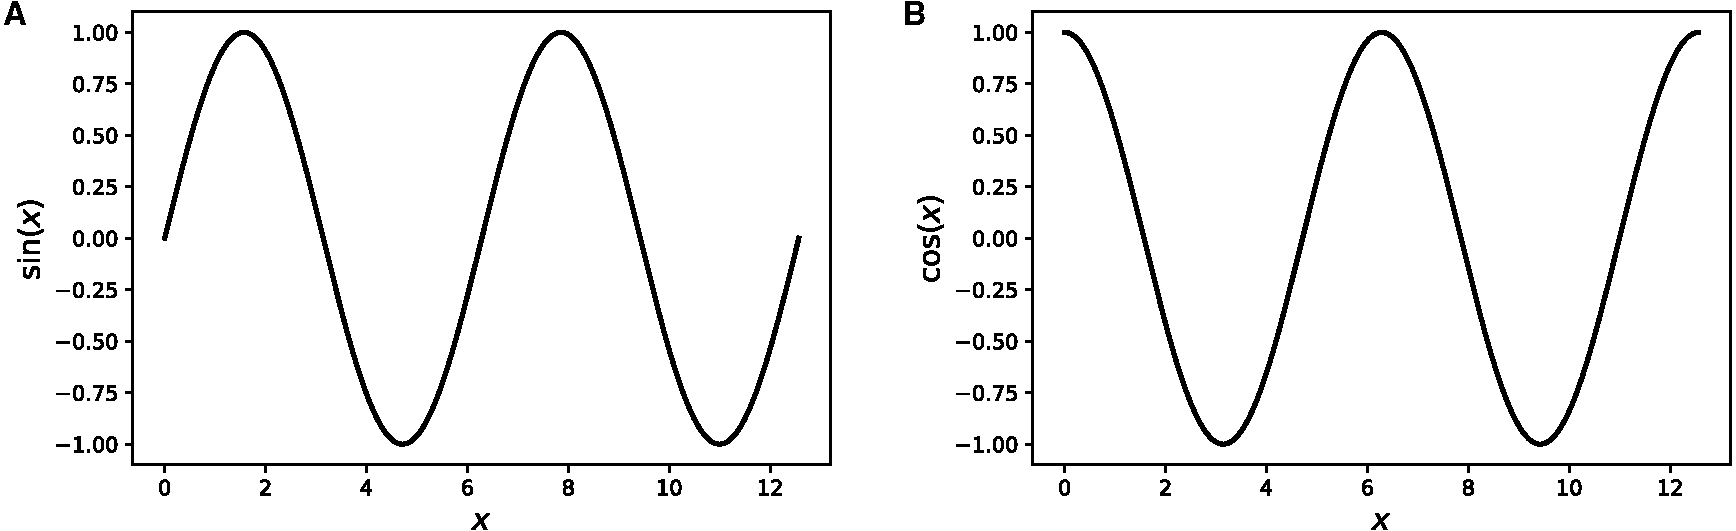
\includegraphics[width=0.6\textwidth]{figs/trig}
\caption{\textbf{Two trigonometric functions, but rendered smaller.  A. Sine wave.} Look at the pretty sine wave!  \textbf{B. Cosine wave.}  The cosine wave looks nice too.  Also see Figure~\demo~in the main text.}
\label{fig:demo}
\end{figure}

\newpage
\renewcommand{\refname}{Supplementary references}
\bibliographystyle{apa}
\bibliography{CDL-bibliography/cdl}



\end{document}
